A primeira etapa deste trabalho é focada em uma contextualização de sistemas dinâmicos instáveis e na necessidade do desenvolvimento de controladores adequados para lidar com tais instabilidades. Esta seção mostra os resultados obtidos nos testes feitos relacionados ao sistema de pêndulo invertido.

Para uma simulação, assumiu-se uma instância do sistema de pêndulo invertido com os seguintes valores definidos para a massa do carro ($M$), massa da haste ($m$) e comprimento da haste ($l$):
\begin{center}
$M$ = 2 kg,\quad$m$ = 0,1 Kg,\quad$l$ = 0,5 m
\end{center}

A \autoref{fig:simulation-pendulum-uncontrolled} mostra a resposta do sistema de pêndulo invertido com os valores definidos a uma entrada em degrau unitário obtida a partir da execução do código mostrado no Apêndice \ref{chap:apendicex-pendulum-modelagem-controle}. Este código é uma variação do presente em \cite[p.~750]{Ogata2010}.

A figura mostra a resposta dos quatro estados do sistema: $\theta$, $\dot{\theta}$, $x$ e $\dot{x}$. Como se pode ver, a resposta de todos os estados à entrada em degrau diverge, mostrando a instabilidade do sistema.

\begin{figure}[!htb]
    \centering
    \caption{Resposta do sistema de pêndulo invertido a uma entrada em degrau unitário}
    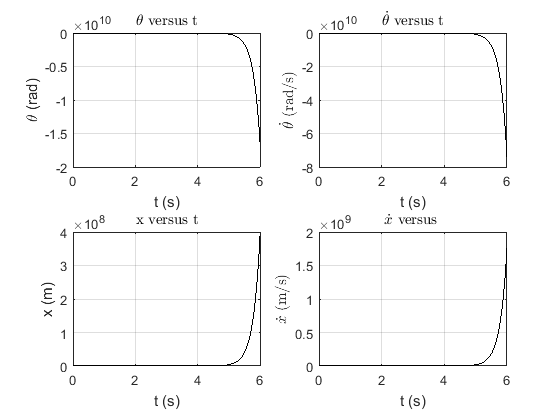
\includegraphics[width=1\textwidth]{./04-figuras/matlab_figuras_pendulo/sistema_sem_controle_estados_black}
    \label{fig:simulation-pendulum-uncontrolled}
\end{figure}

Para mostrar a importância de um sistema adequado de controle, foi implementado, no mesmo código, um controlador da categoria de servo-sistema tipo 1 para o pêndulo invertido. A \autoref{fig:simulation-pendulum-controlled} mostra os quatro estados do sistema também quando submetido a uma entrada em degrau unitário. Desta vez, entretanto, o controlador age e estabiliza o sistema, fazendo que com que ele alcance o estado de equilíbrio. Como se pode ver pela figura, o ângulo $\theta$, bem como sua taxa de variação $\dot{\theta}$, alcançam estabilidade no regime permanente no valor zero indicando que a haste atinge o estado de equilíbrio vertical. Como se pode ver também pela \autoref{fig:simulation-pendulum-controlled}, no gráfico \textit{x versus t}, o carro não volta à posição inicial 0, mas se estabiliza na posição $x=1$, sendo este valor referente à amplitude do sinal em degrau na entrada do sistema. Os gráficos $\dot{\theta}\ versus\ t$ e $\dot{x}\ versus\ t$ mostram a taxa de variação do ângulo da haste e da posição do carro, respectivamente. Como se pode ver, no regime permanente ambos são iguais a zero, indicando estabilidade para ambos os estados.

\begin{figure}[!htb]
    \centering
    \caption{Resposta do sistema de pêndulo invertido a uma entrada em degrau unitário quando controlado por um servo sistema tipo um}
    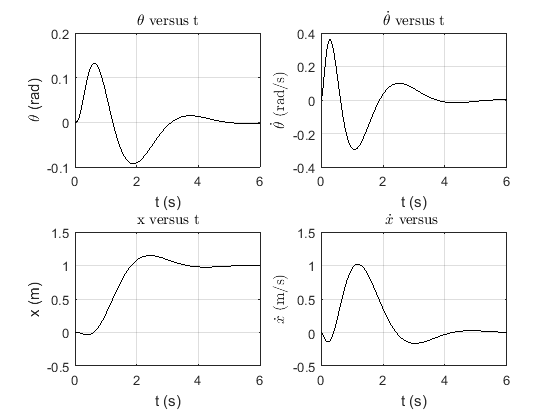
\includegraphics[width=1\textwidth]{./04-figuras/matlab_figuras_pendulo/sistema_com_controle_estados_black}
    \label{fig:simulation-pendulum-controlled}
\end{figure}